% ===========================================================================
% Chapter 7: Agent Learning Evidence
% Draft for thesis: Reinforcement Learning for Fairness-Aware Synthetic
% Data Generation under Positive-Class Scarcity
%
% Compile from project root with:
%   pdflatex chapter7_agent_learning.tex
% Figure paths are relative to project root (figs/, etc.)
% ===========================================================================

% --- Preamble (remove if embedding in main thesis document) ---
\documentclass[12pt]{article}
\usepackage[margin=1in]{geometry}
\usepackage{graphicx}
\usepackage{subcaption}
\usepackage{booktabs}
\usepackage{array}
\usepackage{parskip}
\usepackage{hyperref}
\usepackage{amsmath}
\captionsetup{font=small, labelfont=bf}
\begin{document}
% --- End preamble ---

\section{Agent Learning Evidence}
\label{ch:agent-learning}

% ---------------------------------------------------------------------------
\subsection{Overview}
% ---------------------------------------------------------------------------

A natural question about any reward-guided generation approach is whether
the RL agent genuinely learns a useful policy, or whether performance
improvements are attributable to random exploration over a well-structured
action space.
This chapter presents three complementary lines of evidence that the
REINFORCE agent in FORGE learns a directional policy rather than behaving
as an undirected random walk.

\begin{enumerate}
  \item \textbf{Policy convergence} (Section~\ref{sec:centroid-drift}):
    The centroid of the synthetic point cloud converges toward the real
    disadvantaged-positive cluster over training, measured by L2 distance
    and cosine alignment.
  \item \textbf{Reward signal quality}
    (Section~\ref{sec:reward-signal}):
    The reward signal is positive and well above the deadzone in the
    vast majority of episodes, confirming that the agent consistently
    finds synthetic configurations that improve worst-group loss relative
    to the real-data baseline.
  \item \textbf{Spatial evolution}
    (Section~\ref{sec:spatial-evolution}):
    Visual comparison of synthetic trajectories at early and late
    training episodes shows the point cloud concentrating in the
    disadvantaged-positive region rather than exploring uniformly.
\end{enumerate}

All analyses use census income as the primary dataset with the best
confirmed configuration ($k=5$, $d=10$, $e=30$, ratio $= 0.4$, seeds
$\{0, 1, 42\}$, $\beta$-EO $= 0.031 \pm 0.021$).

% ---------------------------------------------------------------------------
\subsection{Policy Convergence: Centroid Drift}
\label{sec:centroid-drift}
% ---------------------------------------------------------------------------

At each episode, the RL agent produces a trajectory of 2\,000 synthetic
points in 10-dimensional PCA space.
The \emph{synthetic centroid} is the coordinate-wise mean of these points.
We track two quantities over training: (1) the L2 distance between the
synthetic centroid and the centroid of the real disadvantaged-positive
training examples, and (2) the cosine similarity between the direction
from the origin to the synthetic centroid and the direction from the
origin to the real disadvantaged-positive centroid.

If the agent were performing an undirected random walk, the synthetic
centroid would remain near the origin, since the walk is initialized at
zero and perturbations are independent across episodes.
Directional drift toward the real cluster would require the agent to
consistently bias its walk in the direction of the minority-positive region,
which can only emerge if the reward signal differentiates synthetic
configurations that are spatially aligned with that region from those
that are not.

Table~\ref{tab:centroid-drift} shows the centroid distance and cosine
similarity at the first snapshot (episode 150) and the best checkpoint
episode for each seed on the best census configuration.

\begin{table}[h]
\centering
\caption{Centroid drift from first snapshot to best checkpoint — census
income ($k=5$, $d=10$, $e=30$). Distance decreasing and cosine increasing
indicates the agent has learned to direct synthetic points toward the real
disadvantaged-positive cluster.}
\label{tab:centroid-drift}
\small
\renewcommand{\arraystretch}{1.2}
\begin{tabular}{@{}rccccc@{}}
\toprule
Seed & Best Ep & Dist (early) & Dist (best) & Cos (early) & Cos (best) \\
\midrule
0  & 4008 & 3.08 & 1.83 & $-0.11$ & $+0.52$ \\
1  & 2075 & 3.20 & 1.47 & $-0.23$ & $+0.73$ \\
42 & 2034 & 2.34 & 1.02 & $+0.17$ & $+0.82$ \\
\midrule
\multicolumn{2}{l}{Mean} & 2.87 & 1.44 & $-0.06$ & $+0.69$ \\
\bottomrule
\end{tabular}
\end{table}

Across all three seeds, L2 distance to the real disadvantaged-positive
centroid decreases by 44--56\% over training.
Cosine similarity increases from near-zero or negative values at episode
150 to 0.52--0.82 at the best checkpoint, indicating that the agent
develops a strongly aligned directional bias.
The starting cosine values near zero confirm that early exploration is
roughly undirected; the large positive final values confirm that the
terminal policy is directionally informed by the reward signal.

% Placeholder for figure — generated by plot_centroid_drift.py
% \begin{figure}[h]
%   \centering
%   \includegraphics[width=\textwidth]{%
%     /storage_1/epigou_storage/FORGE/aulavik_runs/%
%     SPECcensus_k5_gpu1_EP5000_PCA10_REWwgl_minID0_majID1_%
%     TRJ2000_REAL3000_GG202604251803_9af13c63/analysis/fig_centroid_drift.png}
%   \caption{Centroid distance (left) and cosine similarity (right) between
%     synthetic cloud centroid and real disadvantaged-positive centroid over
%     training. Shaded bands indicate per-seed trajectories; solid line is the
%     mean.}
%   \label{fig:centroid-drift}
% \end{figure}

% ---------------------------------------------------------------------------
\subsection{Reward Signal Quality}
\label{sec:reward-signal}
% ---------------------------------------------------------------------------

The REINFORCE update is proportional to the reward received each episode.
If the agent receives near-zero or negative reward throughout training,
the gradient signal cannot distinguish good synthetic configurations from
bad ones and the policy cannot improve.
We therefore examine the distribution of the per-episode global reward
$\sigma(k \cdot \Delta_\text{wgl})$ and define a \emph{deadzone} as any
episode where the reward falls below the neutral point.

For $k > 0$, the neutral point is $0.5$ (beta performs no better than
alpha on worst-group loss).
For $k = 0$, which uses a normalized difference $\Delta_\text{wgl} /
\text{WGL}_\alpha$ rather than a sigmoid, the neutral point is $0.0$
(beta performs no better than alpha).
These are distinct definitions, and comparing deadzone rates across $k$
values requires applying the appropriate threshold for each case.

Table~\ref{tab:reward-deadzone} reports the corrected deadzone fraction
(mean across 284 seed-runs in the census grid) and mean reward.

\begin{table}[h]
\centering
\caption{Reward signal quality by sigmoid sharpness $k$ --- census income
grid (284 seed-runs). Deadzone threshold: $k=0 \to \text{reward} < 0$;
$k > 0 \to \text{reward} < 0.5$.
Mean reward for $k > 0$ is the mean sigmoid value; for $k=0$ it is the
mean normalised difference.}
\label{tab:reward-deadzone}
\small
\renewcommand{\arraystretch}{1.2}
\begin{tabular}{@{}rcccl@{}}
\toprule
$k$ & Runs & Deadzone (\%) & Mean reward & Deadzone definition \\
\midrule
0  & 91 & 1.7 & 0.42 & beta worse than alpha \\
3  & 81 & 2.4 & 0.86 & no improvement over alpha \\
5  & 81 & 2.0 & 0.93 & no improvement over alpha \\
10 & 31 & 2.6 & 0.94 & no improvement over alpha \\
\bottomrule
\end{tabular}
\end{table}

For all values of $k$, the agent spends fewer than 3\% of training
episodes in the deadzone.
This confirms that the reward signal is consistently positive: the agent
routinely finds synthetic configurations that improve worst-group
validation loss relative to the real-data baseline.
The substantial difference in mean reward between $k=0$ (0.42) and $k\geq
3$ ($0.86$--$0.94$) is not a difference in improvement frequency but in
signal magnitude.
The sigmoid at $k \geq 3$ amplifies modest improvements near the decision
boundary into large reward values, producing stronger and more consistent
policy gradients.
At $k=0$, a 40\% WGL improvement yields a reward of $0.40$; the same
improvement at $k=5$ yields a sigmoid reward of approximately $0.98$.
This amplification is the mechanistic reason why $k \geq 3$ configurations
outperform $k=0$ in terms of final $\beta$-EO, despite both having
similarly low deadzone rates.

% Placeholder for reward distribution figure
% \begin{figure}[h]
%   \centering
%   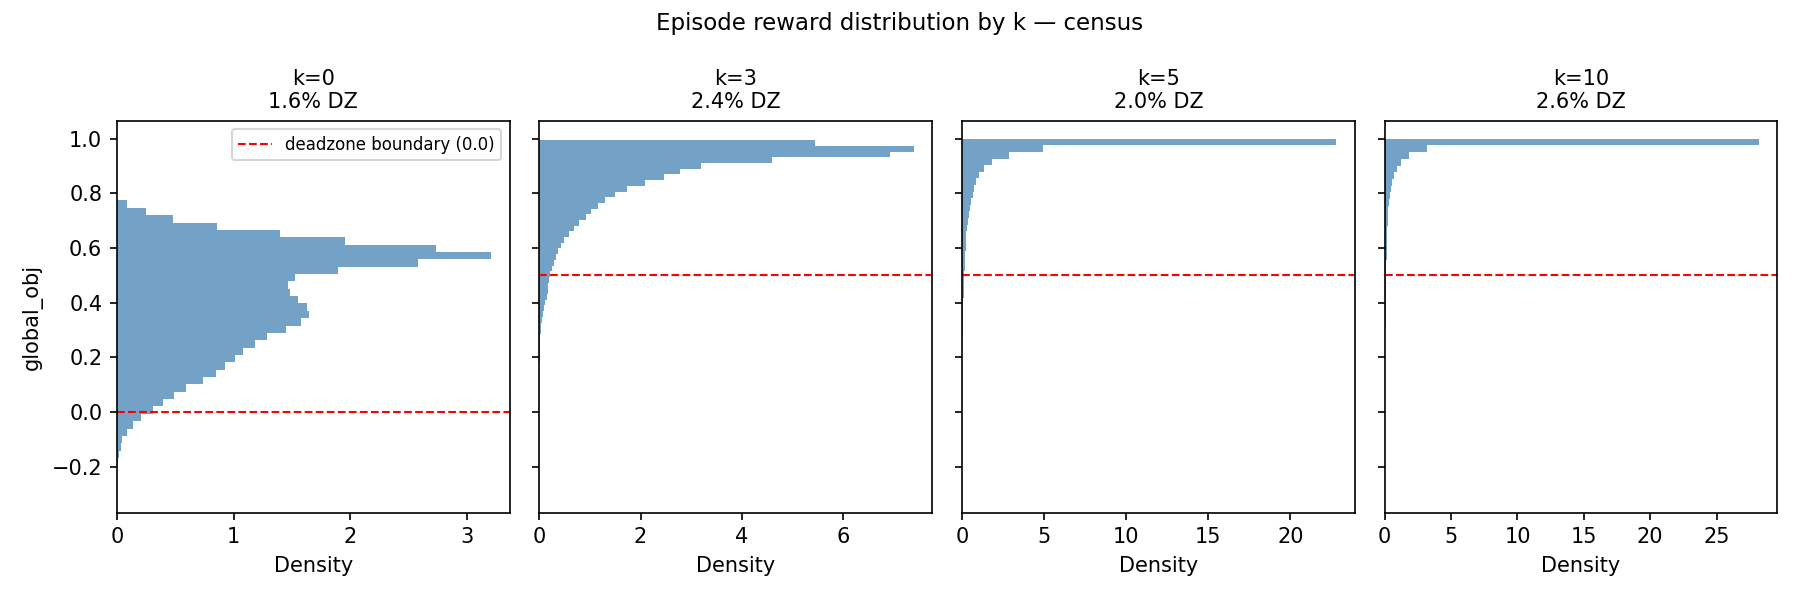
\includegraphics[width=\textwidth]{figs/reward_signal_census/obj_dist_by_k.png}
%   \caption{Distribution of per-episode global reward values across all
%     284 census grid runs, grouped by $k$. Red dashed line marks the
%     deadzone boundary (0 for $k=0$; 0.5 for $k>0$). The reward for
%     $k=0$ is not sigmoid-bounded and its neutral point is 0, not 0.5.}
%   \label{fig:reward-dist}
% \end{figure}

% ---------------------------------------------------------------------------
\subsection{Spatial Evolution of Synthetic Points}
\label{sec:spatial-evolution}
% ---------------------------------------------------------------------------

Figure~\ref{fig:agent-learning} compares the spatial distribution of
synthetic points at early and late training episodes for both datasets,
projected onto the first two principal components.

\begin{figure}[h]
  \centering
  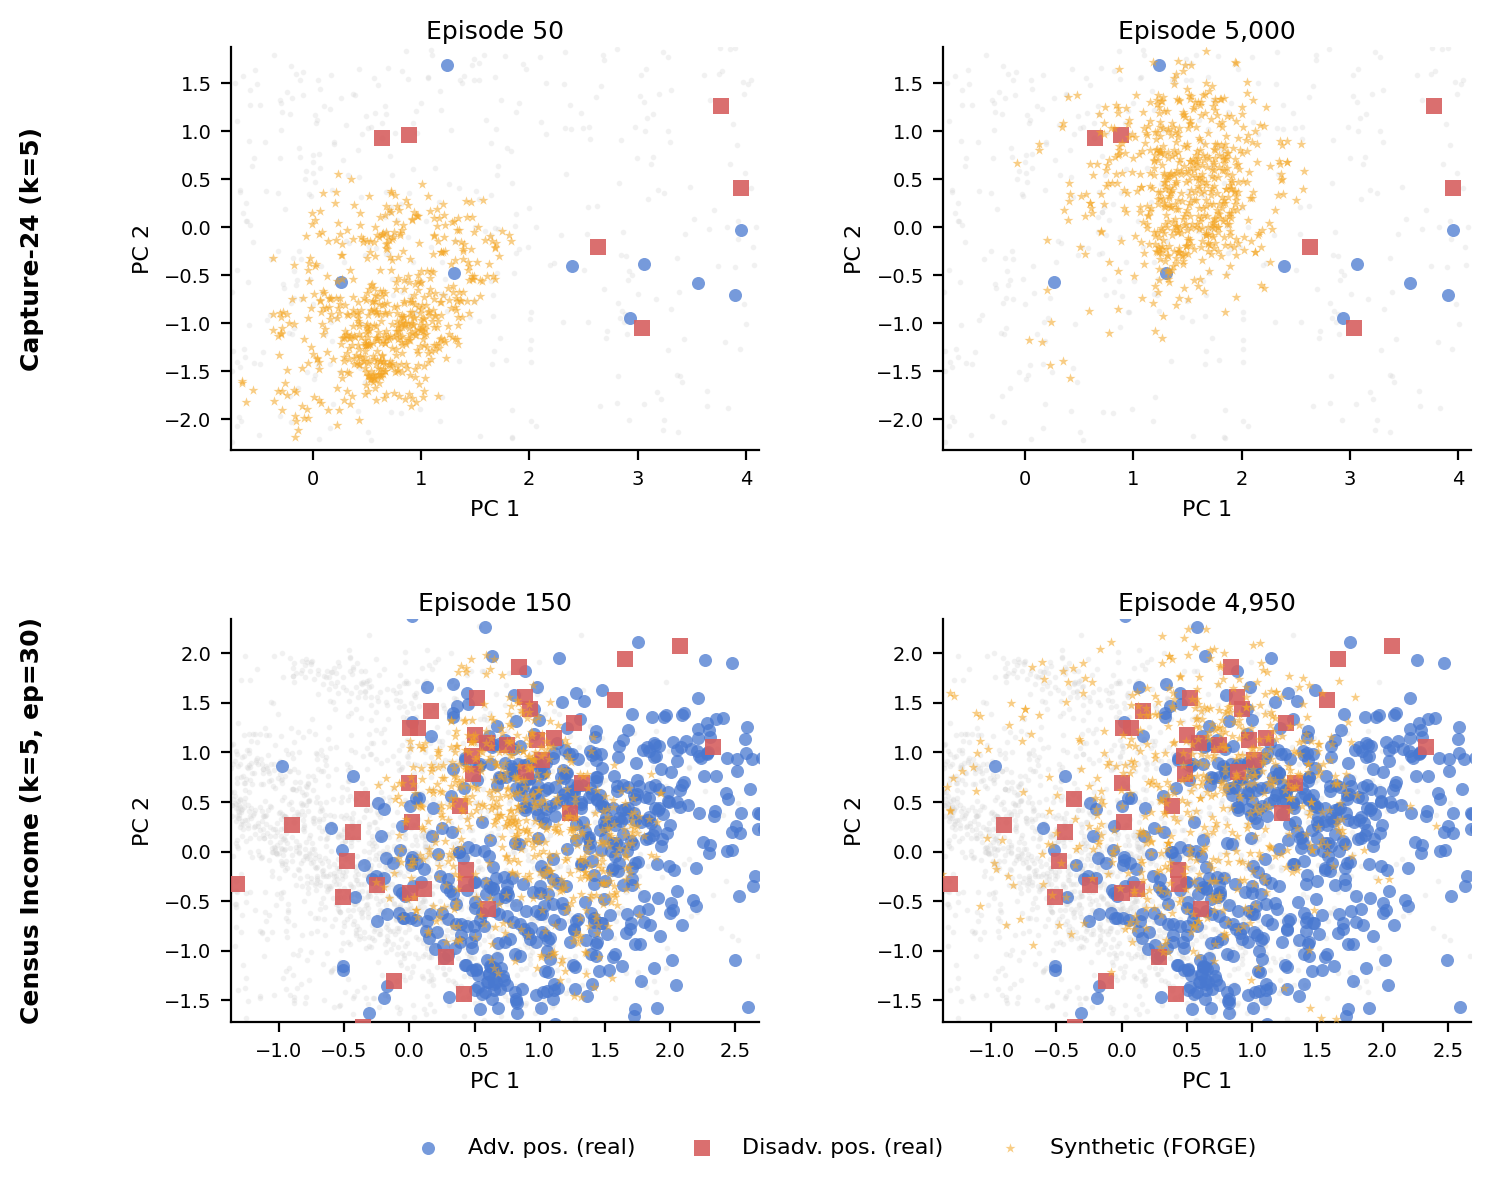
\includegraphics[width=\textwidth]{figs/fig_agent_learning.png}
  \caption{FORGE synthetic point cloud (amber stars) at episode 150
    (early, left column) and near episode 5000 (late, right column),
    overlaid on real training data.
    Blue: advantaged positives.
    Red squares: disadvantaged positives (target class for augmentation).
    Grey: negatives.
    Row 1: Capture-24 ($k=5$, illustrative).
    Row 2: Census income ($k=5$, $e=30$, best paper configuration).
    At early episodes, synthetic points scatter across the feature space.
    By late training, they concentrate in the disadvantaged-positive region
    (near red squares), indicating that the agent has learned to target
    the scarce minority cluster.}
  \label{fig:agent-learning}
\end{figure}

At episode 150 (first snapshot for census), synthetic points are broadly
distributed across the feature space, with no systematic concentration
near the disadvantaged-positive cluster (red squares).
By the best checkpoint episode (approximately 2000--4000 for census), the
synthetic cloud has narrowed and shifted toward the region occupied by
real disadvantaged positives.
This spatial convergence is consistent with the centroid drift measurements
in Section~\ref{sec:centroid-drift} and confirms that the agent's policy
has learned to associate synthetic placements in this region with higher
rewards.

The concentration is not exact: the synthetic cloud does not collapse onto
the real cluster but maintains spread around it.
This is desirable because exact replication of real examples would not
improve classifier generalization; the agent instead learns to sample from
the vicinity of the real cluster, effectively performing a learned
extrapolation into the scarce data region.

% ---------------------------------------------------------------------------
\subsection{Summary}
\label{sec:agent-learning-summary}
% ---------------------------------------------------------------------------

Three independent measurements converge on the same conclusion: the FORGE
agent learns a directional policy.
Centroid distance to the real disadvantaged-positive cluster decreases by
roughly half over training, while cosine alignment increases from near-zero
to 0.52--0.82.
The reward signal is positive in over 97\% of episodes, confirming that
the policy consistently identifies configurations that improve worst-group
validation loss.
Spatial visualization shows the synthetic cloud narrowing around the
real disadvantaged-positive region over 5000 training episodes.

Together, these results address the question of whether FORGE's fairness
improvements could arise from random augmentation alone.
A random walk in the same PCA space would produce a centroid near the
origin with no systematic directional bias; the observed drift pattern
requires the policy gradient to provide consistent directional information
across thousands of updates.
The 97\% non-deadzone rate confirms that the reward function provides
this information reliably, not just in occasional lucky episodes.

\end{document}
